\subsection{Short introduction to parallel Haskells}
\label{sec:parallelHaskells}
\label{sec:parEvalNIntro}
In its purest form, parallel computation (on functions) can be looked at as the execution of some functions |a -> b| in parallel or |parEvalN :: [a -> b] -> [a] -> [b]|, as also Figure~\ref{fig:parEvalN} symbolically shows.
\begin{figure}[t]
  \centering
	\includegraphics[scale=0.7]{images/parEvalN}
	\caption{Schematic illustration of |parEvalN|. A list of inputs is transformed by different functions in parallel.}
	\label{fig:parEvalN}
\end{figure}

In this section, we will implement this non-Arrow version which will later be adapted for usage in our Arrow-based parallel Haskell.

There exist several parallel Haskells already. Among the most important are probably GpH \citep[based on |par| and |pseq| \enquote{hints},][]{Trinder1996,Trinder1998a}, the |Par| Monad \citep[a monad for deterministic parallelism,][]{par-monad,Foltzer:2012:MPC:2398856.2364562}, Eden \citep[a parallel Haskell for distributed memory,][]{eden,Loogen2012}, HdpH \citep[a Template Haskell-based parallel Haskell for distributed memory,][]{Maier:2014:HDS:2775050.2633363,stewart_maier_trinder_2016} and LVish \citep[a |Par| extension with focus on communication,][]{Kuper:2014:TPE:2666356.2594312}.

As the goal of this paper is not to re-implement yet another parallel runtime, but to represent parallelism with Arrows, we base our efforts on existing work which we wrap as backends behind a common interface. For this paper we chose GpH for its simplicity, the |Par| Monad to represent a monadic DSL, and Eden as a distributed parallel Haskell.

LVish and HdpH were not chosen as the former does not differ from the original |Par| Monad with regard to how we would have used it in this paper, while the latter (at least in its current form) does not comply with our representation of parallelism due to its heavy reliance on Template Haskell.

We will now go into some detail on GpH, the |Par| Monad and Eden, and also give their respective implementations of the non-Arrow version of |parEvalN|.

%Before we go into detail on how we can use this idea of parallelism
%for parallel Arrows, as a short introduction to parallelism in
%Haskell we will now implement |parEvalN| with several different
%parallel Haskells.

\subsubsection{Glasgow parallel Haskell -- GpH}
\label{sec:GpHIntro}
GpH \cite{Marlow2009,Trinder1998a} is one of the simplest ways to do parallel processing found in standard GHC.\footnote{The Multicore implementation of GpH is available on Hackage under \url{https://hackage.haskell.org/package/parallel-3.2.1.0}, compiler support is integrated in the stock GHC.} Besides some basic primitives (|par| and |pseq|), it ships with parallel evaluation strategies for several types which can be applied with |using :: a -> Strategy a -> a|, which is exactly what is required for an implementation of |parEvalN|.


\begin{code}
parEvalN :: (NFData b) => [a -> b] -> [a] -> [b]
parEvalN fs as = let bs = zipWith ($) fs as 
                 in bs `using` parList rdeepseq
\end{code} %$

In the above definition of |parEvalN| we just apply the list of functions |[a -> b]| to the list of inputs |[a]| by zipping them with the application operator |$|. % $
We then evaluate this lazy list |[b]| according to a |Strategy [b]| with the |using :: a -> Strategy a -> a| operator. We construct this strategy with |parList :: Strategy a -> Strategy [a]| and |rdeepseq :: NFData a => Strategy a| where the latter is a strategy which evaluates to normal form. Other strategies like e.g. evaluation to weak head normal form are available as well. It also allows for custom |Strategy| implementations to be used.
%
Fig.~\ref{fig:parEvalNMulticoreImg} shows a visual representation of this code.

% \begin{figure}[h]
% \begin{code}
% parEvalN :: (NFData b) => [a -> b] -> [a] -> [b]
% parEvalN fs as = let bs = zipWith ($) fs as 
%                  in (bs `using` parList rdeepseq)
% \end{code}
% \caption{Multicore version of |parEvalN|.}
% \label{fig:parEvalNMulticore}
% \end{figure}

\begin{figure}[t]
	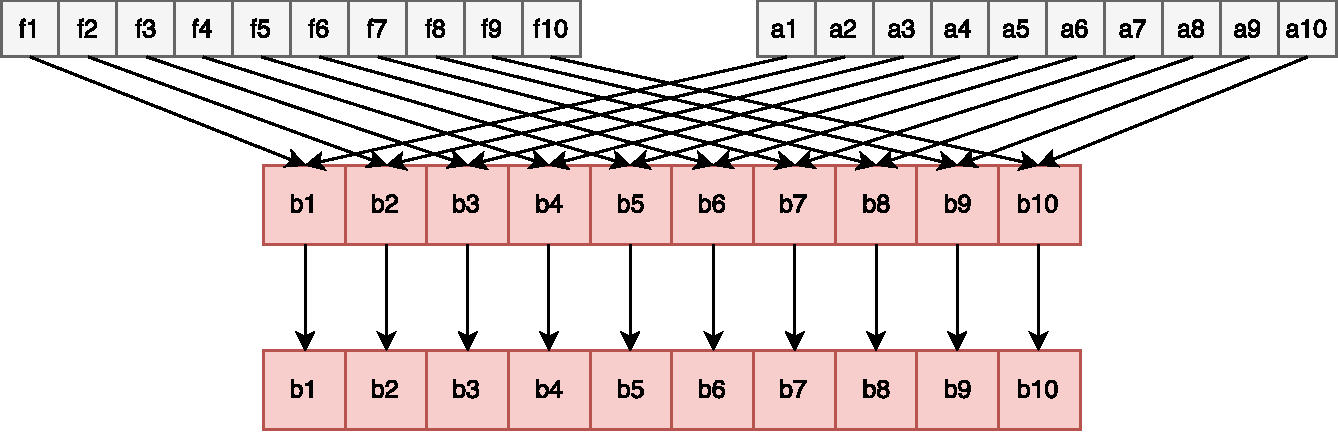
\includegraphics[scale=0.5]{images/parEvalNMulticore}
	\caption{|parEvalN| (GpH).}
	\label{fig:parEvalNMulticoreImg}
\end{figure} %$ %% formatting

\subsubsection{|Par| Monad}
The |Par| Monad\footnote{The |Par| monad can be found in the \texttt{monad-par} package on Hackage under \url{https://hackage.haskell.org/package/monad-par-0.3.4.8/}.} introduced by \citet{par-monad}, is a Monad designed for composition of parallel programs. Let:

\begin{code}
parEvalN :: (NFData b) => [a -> b] -> [a] -> [b]
parEvalN fs as = runPar $ 
	(sequenceA (map (return . spawn) (zipWith ($) fs as))) >>= mapM get
\end{code}

The |Par| Monad version of our parallel evaluation function |parEvalN| is defined by zipping the list of |[a -> b]| with the list of inputs |[a]| with the application operator |$| just like with GpH. % $
Then, we map over this not yet evaluated lazy list of results |[b]| with |spawn :: NFData a => Par a -> Par (IVar a)| to transform them to a list of not yet evaluated forked away computations |[Par (IVar b)]|, which we convert to |Par [IVar b]| with |sequenceA|. We wait for the computations to finish by mapping over the |IVar b| values inside the |Par| Monad with |get|. This results in |Par [b]|. We execute this process with |runPar| to finally get |[b]|. While we used |spawn| in the definition above, a head-strict variant can easily be defined by replacing |spawn| with |spawn_ :: Par a -> Par (IVar a)|.
Fig.~\ref{fig:parEvalNParMonadImg} shows a graphical representation.

% \begin{figure}[h]
% \begin{code}
% parEvalN :: (NFData b) => [a -> b] -> [a] -> [b]
% parEvalN fs as = runPar $ 
% 	(sequenceA $ map (spawnP) $ zipWith ($) fs as) >>= mapM get
% \end{code}
% \caption{|Par| Monad version of |parEvalN|.}
% \label{fig:parEvalNParMonad}
% \end{figure}
\begin{figure}[t]
	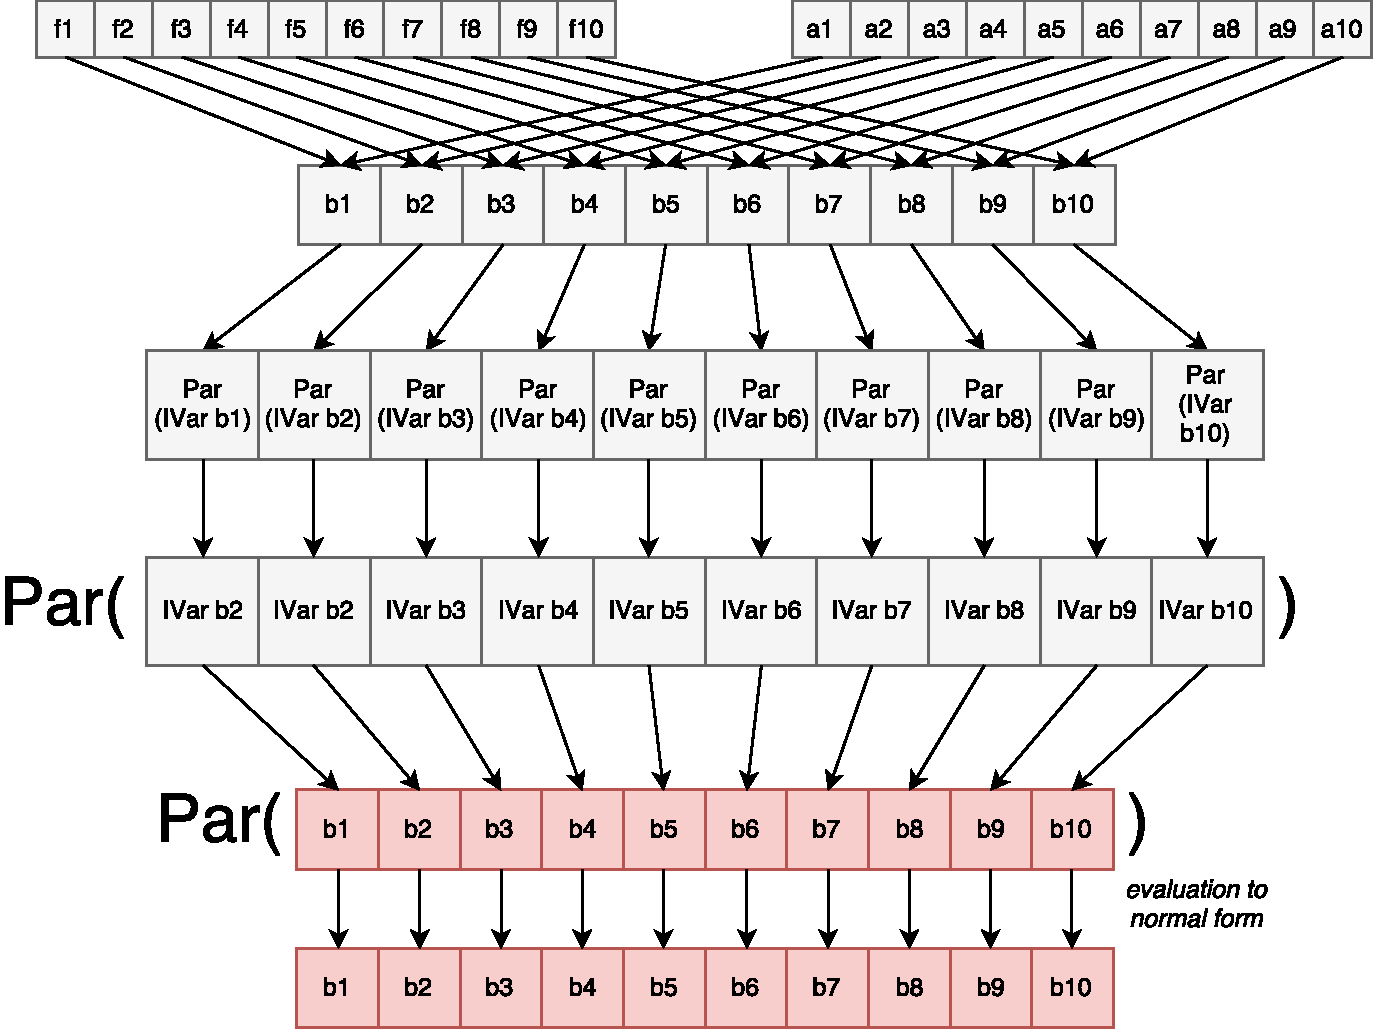
\includegraphics[scale=0.5]{images/parEvalNParMonad}
	\caption{|parEvalN| (|Par| Monad).}
	\label{fig:parEvalNParMonadImg}
\end{figure}

\subsubsection{Eden}
Eden \cite{eden,Loogen2012} is a parallel Haskell for distributed memory and comes with MPI and PVM as distributed backends.\footnote{The projects homepage can be found at \url{http://www.mathematik.uni-marburg.de/~eden/}. The Hackage page is at \url{https://hackage.haskell.org/package/edenmodules-1.2.0.0/}.} It is targeted towards clusters, but also functions well in a shared-memory setting with a further simple backend. However, in contrast to many other parallel Haskells, in Eden each process has its own heap. This seems to be a waste of memory, but with distributed programming paradigm and individual GC per process, Eden yields good performance results on multicores, as well \cite{arcs-dc,aswad2009low}.

While Eden comes with a Monad |PA| for parallel evaluation, it also ships with a completely functional interface that includes
%\\
a |spawnF :: (Trans a, Trans b) => [a -> b] -> [a] -> [b]|
%\\
%a |spawnF| 
function that
%This 
allows us to define |parEvalN| directly:

\begin{code}
parEvalN :: (Trans a, Trans b) => [a -> b] -> [a] -> [b]
parEvalN = spawnF 
\end{code}
% \begin{figure}[h]
% 	\includegraphics[scale=0.5]{images/parEvalNEden}
% 	\caption{Dataflow of the Eden |parEvalN| version.}
% 	\label{fig:parEvalNEden}
% \end{figure}
% A simplistic graphical depiction of this definition can be found in Fig.~\ref{fig:parEvalNEden}.

\paragraph{Eden TraceViewer.}
\label{sec:edentv}
To comprehend the efficiency and the lack thereof in a parallel program, an inspection of its execution is extremely helpful. While some large-scale solutions exist \cite{Geimer2010}, the parallel Haskell community mainly utilises the tools Threadscope \cite{Wheeler2009} and Eden TraceViewer\footnote{See \url{http://hackage.haskell.org/package/edentv} on Hackage for the last available version of Eden TraceViewer.} \cite{Berthold2007a}. In the next sections we will present some \emph{trace visualisations}, the post-mortem process diagrams of Eden processes and their activity.

The trace visualisations are colour-coded. In such a visualisation (Fig.~\ref{fig:withoutFutures}), the $x$ axis shows the time, the $y$ axis enumerates the machines and processes. The visualisation shows a running process in green, a blocked process is red. If the process is \enquote{runnable}, \ie it may run, but does not, it is yellow. The typical reason for this is GC. An inactive machine, where no processes are started yet, or all are already terminated, shows as a blue bar. A~communication from one process to another is represented with a black arrow. A~stream of communications, \eg a transmitted list is shows as a dark shading between sender and receiver processes.


%%% Local Variables:
%%% mode: latex
%%% TeX-master: "main"
%%% End:
